\chapter{Úvod}

Dungeon Master je počítačová hra žánru RPG (role playing game) vyvinuta firmou Faster Then Light v roce 1987.
Byla to první real-time hra tohoto typu s pseudo 3D pohledem a ovládáním pomocí myši. Hráč má k dispozici skupinu až čtyř hrdinů,
s kterými prochází podzemní bludiště a bojuje s nepřáteli \cc{obr0:uvod}. Tito hrdinové se ve hře nazývají šampioni a mohou se 
zdokonalovat v různých dovednostech. 

\begin{figure}[H]\centering
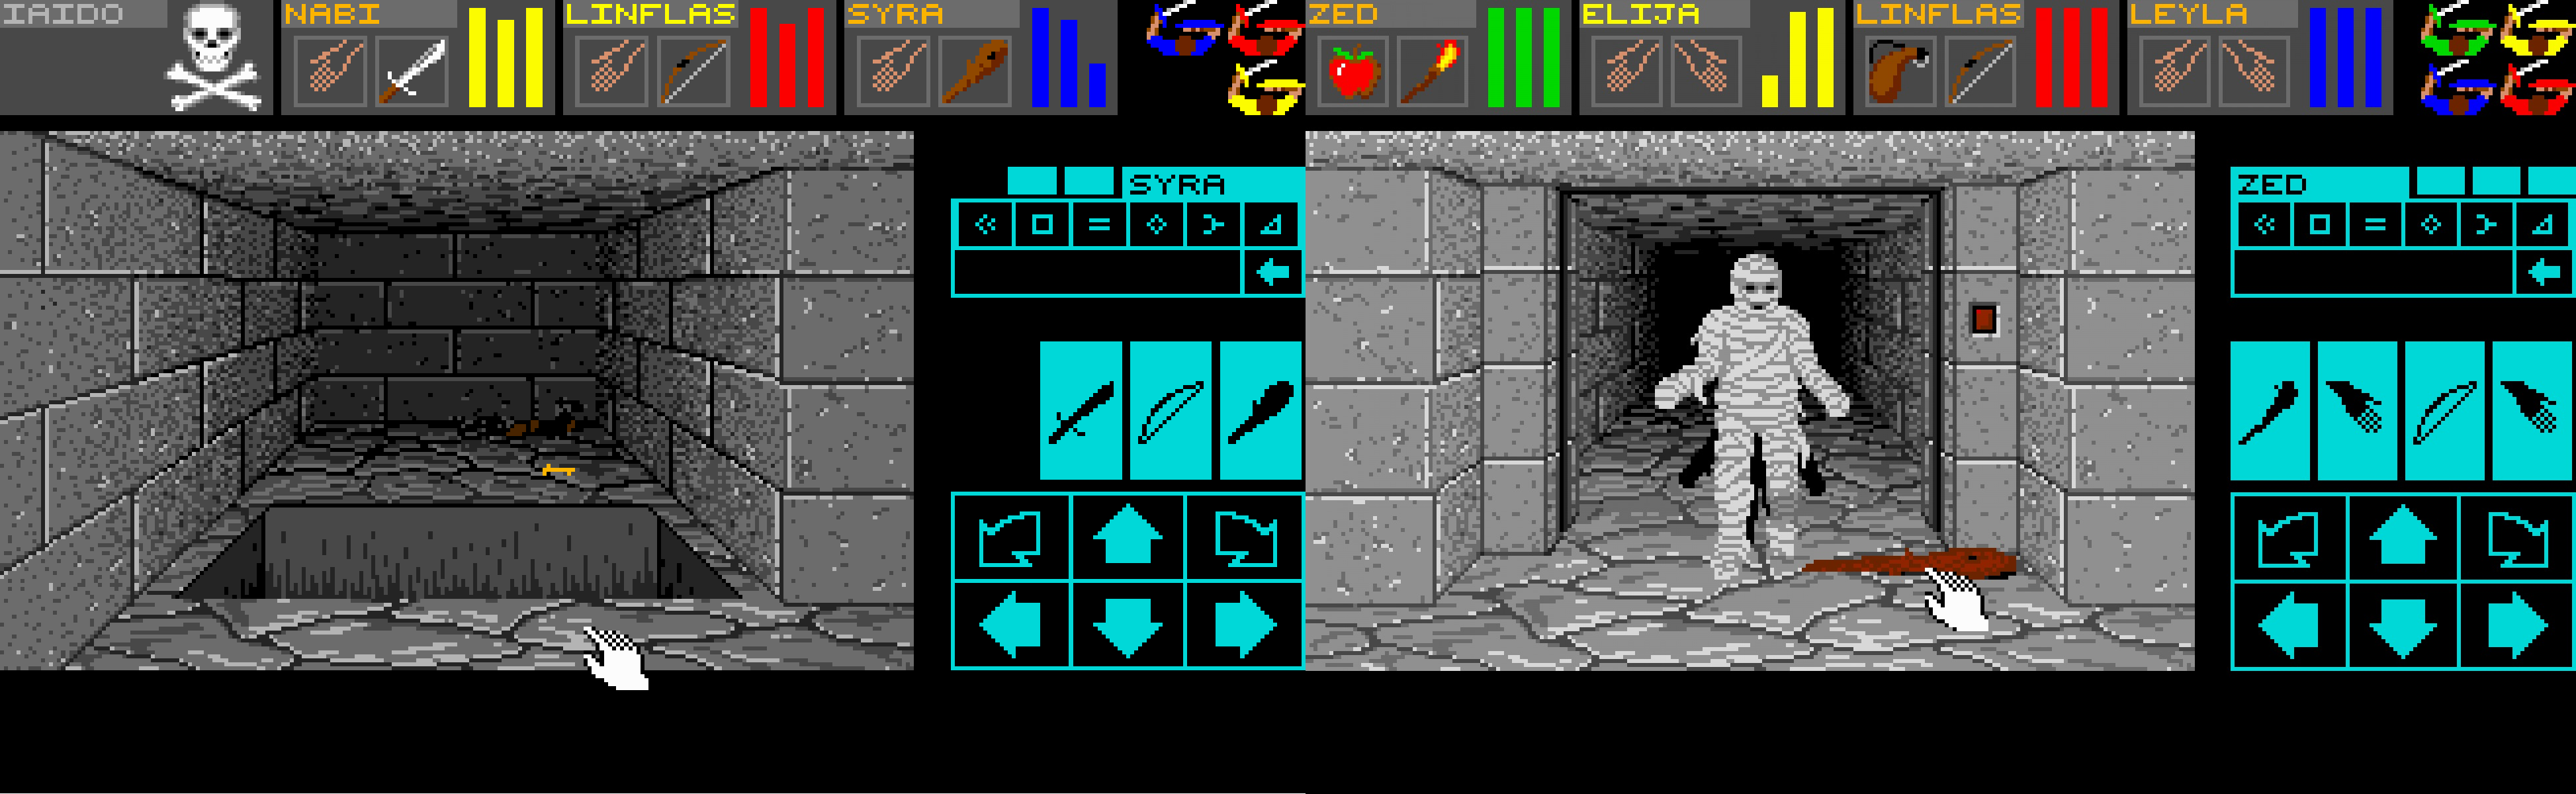
\includegraphics[width=\textwidth]{./img/DM-original-screen.png}
\caption{Screenshot originální hry Dungeon Master}
\label{obr0:uvod}
\end{figure}

Bludiště se skládá z několika úrovní uspořádaných vertikálně pod sebou. 
Jednotlivé úrovně pak nemusí být stejně velké a mohou být od sebe různě horizontálně odsazené.
Každá úroveň je tvořena obdélníkovou plochou s pravidelnou mřížkou \cc{DM-levels}. Pole vymezena mřížkou nazýváme dlaždice a je jich 
ve hře několik typů, které definují jejích vzhled a funkci. Některé dlaždice lze aktivovat tzv. přepínači. Takové typy dlaždic
jsou například dveře nebo jáma \cc{obr0:uvod}, které lze takto otvírat či zavírat. Přepínače mohou být buď nášlapné na podlaze nebo aktivovatelné
pomocí myši na zdech. Mezi úrovněmi lze sestupovat pomocí dlaždic typu schody.  Dále je možné se teleportovat mezi dlaždicemi, a to i v různých úrovních, pomocí dlaždice
typu teleport. 

\imgx{DM-levels}{Ilustrace uspořádání herních úrovní.}

Hráč je na začátku postaven do nejvýše položené úrovně, kde si vybere svoji skupinu šampionů. 
Pohyb skupiny mezi dlaždicemi je zcela diskrétní, to znamená, že se nelze se skupinou zastavit mezi dlaždicemi, ale pohyb je vždy dokončen
až na vedlejší dlaždici. Se skupinou je tedy vždy asociována pouze jedna dlaždice. Na dlaždicích pak mohou
být různé předměty, které je možné sbírat. Šampioni mohou s předměty provádět různé akce.
Například se zbraněmi lze bojovat nebo lektvary je možné pít a zlepšit si tak dočasně vlastnosti. Kromě těchto 
akcí může ještě šampion vyvolávat kouzla. Nicméně k tomu potřebuje dostatečnou úroveň odpovídající dovednosti.
Tímto způsobem je možné vytvářet lektvary nebo vyvolávat útočná či obraná kouzla.

Ve hře je celá řada nepřátelský entit. Liší se vzhledem, útokem a pohybem. Pohyb některých entit 
probíhá ještě po hustší mřížce než jsou dlaždice. Každá entita má definovaný prostor dlaždice, který zaujímá. Je to buď prostor
celé dlaždice, polovina či čtvrtina. \cc{obr2:uvod} Pohyb entit je potom opět diskrétní jako v případě hráčovi skupiny, 
ale tentokrát mezi definovanými částmi dlaždic. 

\begin{figure}[H]\centering
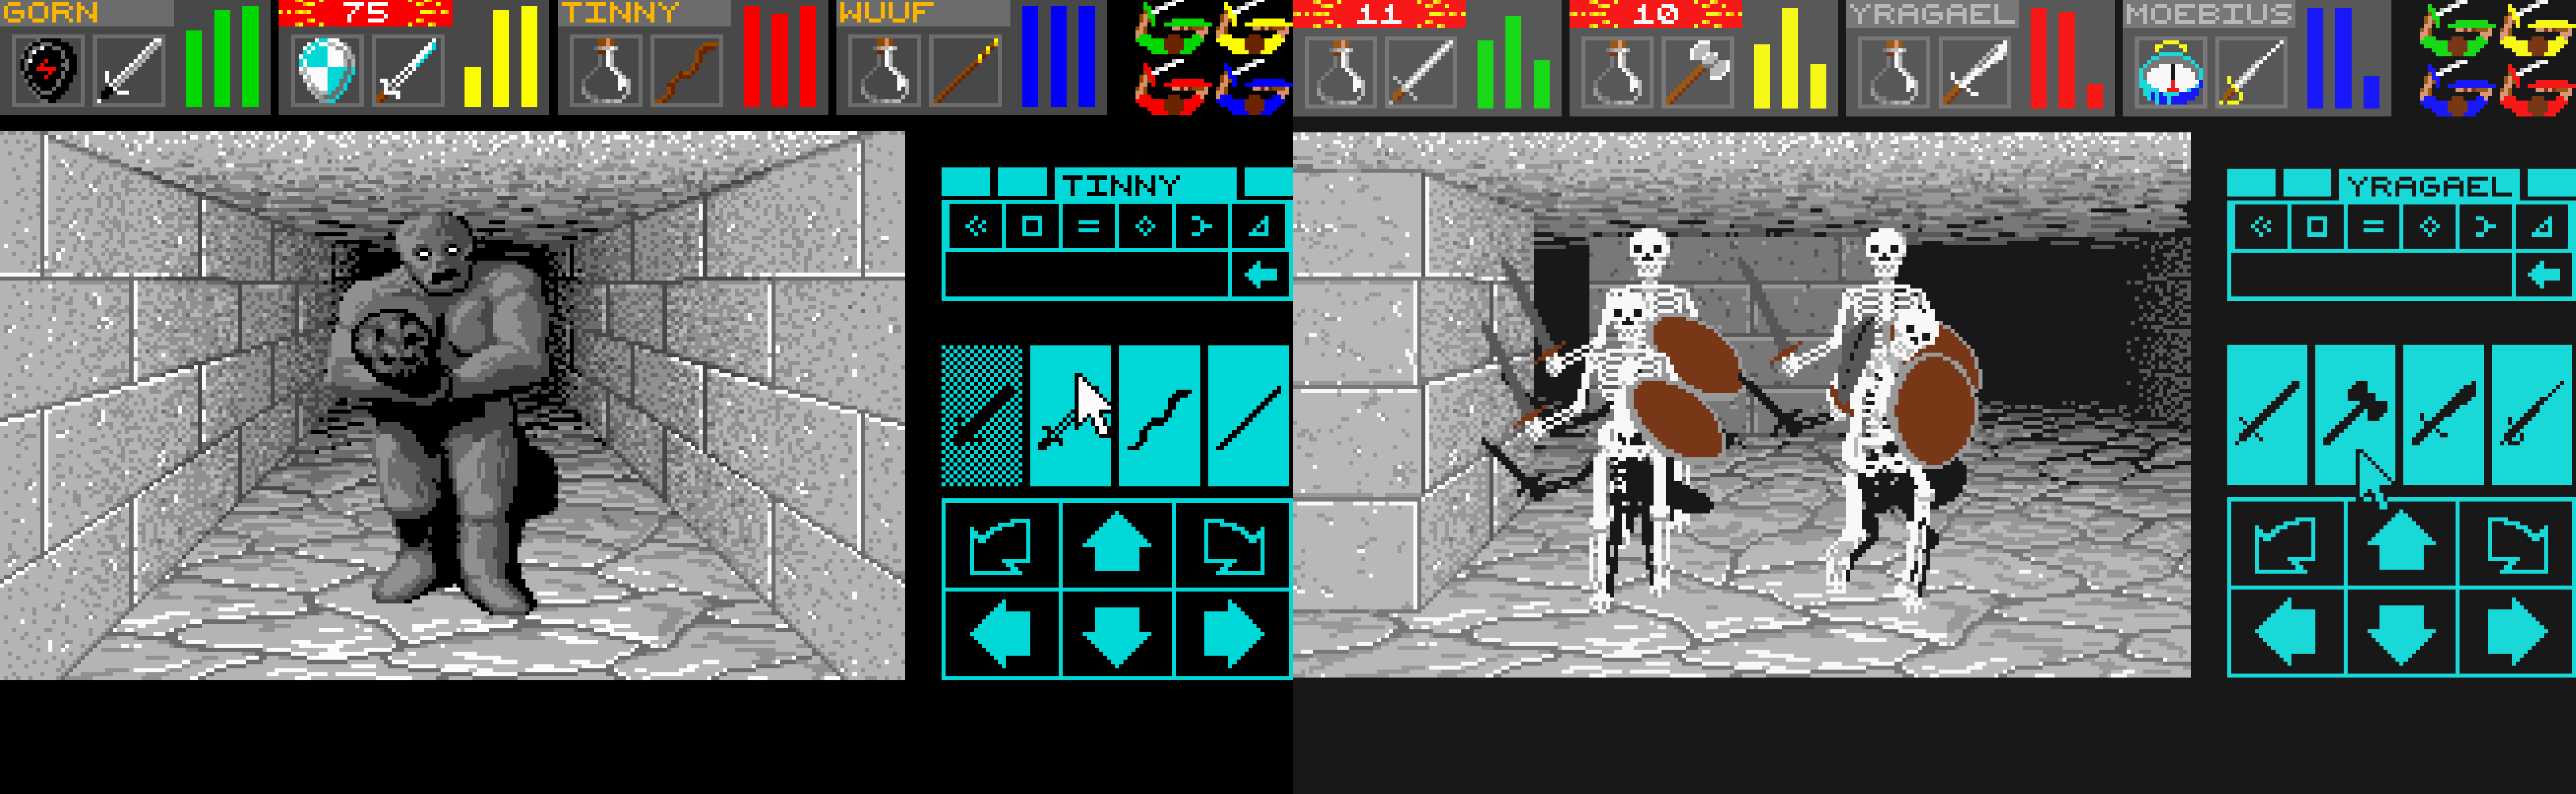
\includegraphics[width=\textwidth]{./img/DM-group-example.png}
\caption{Ilustrace prostorů zaujímaných entitami.}
\label{obr2:uvod}
\end{figure}

\section{Reimplementace Dungeon Masteru}

Výsledkem reimplementace má být engine vhodný pro výuku jazyka C\#. Z tohoto důvodu je nutné, aby byl jazyk C\#
použit pro implementaci enginu. Jelikož C\# je objektově orientovaný jazyk,
je třeba, aby výsledný engine měl dobrý objektový návrh, který bude sloužit jako vhodný materiál k jeho výuce. 
Díky tomu by mělo být možné vytvářet úlohy pro studenty, v kterých by si mohli doimplementovat další funkce enginu nad rámec této práce,
a tak si vyzkoušet objektově orientované programování v praxi. Proto by také mělo být možné
pro engine jednoduše dodělat komponentu, která by prováděla odlišný výstup enginu, díky kterému by mohli být 
úkoly kontrolované například formou CodExu (Code Examinator).

Pro využití enginu způsobem popsaném v předchozím odstavci, je tedy zejména nutné, aby engine obsahoval
podporu pro herní mechaniky hry Dungeon Master -- které by pak bylo možné rozšiřovat.  Následkem toho musí engine obsahovat komponentu 
pro převedení vstupních dat z originální hry na odpovídající herní úrovně. Kromě toho je třeba poskytnout mechanismus,
kterým bude možné dodávat vlastní implementace těchto komponent. V poslední řadě je nutné oddělit výstup enginu do~zvláštní vrstvy,
aby ji bylo možné taktéž jednoduše změnit poskytnutím nové implementace. 

\section{Cíle}

Cílem této práce je tedy vytvořit engine pro hru Dungeon Master, tak aby splňovala následující požadavky:
\begin{enumerate}[label=\textbf{C\arabic*}]
\item Engine bude naprogramovaný v jazyce C\#.
\item\label{aim-mechanics} Engine bude obsahovat podporu pro funkce a mechaniky vyskytující se ve hře Dungeon Master.
\item\label{aim-extensibility} Bude kladen důraz na dobrý objektový návrh, tak aby byl engine co nejlépe rozšiřitelný a bylo 
	tak možné do enginu dodávat jednoduše nové funkce.
\item\label{aim-builders} Engine bude schopný sestavit herní úrovně podle vstupních dat použitých v originální hře. Nicméně
	bude také poskytovat možnost, dodělat si podporu pro jiné formáty.
\item\label{aim-rendering} Engine bude obsahovat oddělenou zobrazovací vrstvu, tak aby mohl být její výstup jednoduše změněn.
\item Projekt bude cílený pro vzdělávaní, tak aby si studenti mohli vyzkoušet do enginu doprogramovat další funkce.
\end{enumerate}
